\chapter{Computabilità}
  In questa sezione si cercherà di rispondere alla domanda: quali problemi possono essere affrontati e risolti mediante gli automi analizzati?
  Si ricordi che automi e grammatiche, pur essendo modelli matematici, si possono considerare dispositivi meccanici per la risoluzione di problemi e che esistono formalismi che hanno un potere espressivo maggiore di altri, ossia sono in grado di riconoscere una classe di linguaggi che altri formalismi non riescono a riconoscere. Inoltre, si ricordi che, nessun formalismo è più potente delle macchine di Turing, sia dal punto di vista del riconoscimento che della traduzione di linguaggi e, per tanto, sono detti formalismi massimi.

  \section{Formalizzazione dei Problemi}
  Molti problemi possono essere opportunamente descritti come il riconoscimento di un determinato linguaggio o come la sua traduzione in un altro linguaggio. Ogni problema matematico è descrivibile mediante una di queste forme, alla sola condizione che il dominio di tale problema sia un insieme numerabile, in maniera tale che i suoi elementi si possono porre in corrispondenza biunivoca con gli elementi di \(\mathbb N\) o, se si preferisce, di \(V^*\), in cui \(V\) rappresenta un alfabeto. Dunque, il problema di origine si può riformulare come il problema di calcolo di una funzione \(f:\mathbb N\to\mathbb N\). Quanto detto è in perfetto accordo con tutti i formalismi matematici esaminati fino ad ora: questi, infatti, sono discreti e hanno un dominio matematico numerabile.

  Il riconoscimento di linguaggi e la loro traduzione sono due formulazioni differenti di un problema, che sono facilmente riducibili l'uno all'altro. Infatti, il problema di stabilire se una determinata stringa \(x\) appartenga o meno al linguaggio \(L\) può anche essere impostato come la traduzione \(\tau_L(x)\), per cui \(\tau_L(x) = 1\) se \(x\in L\), \(\tau_L(x)=0\) altrimenti. Viceversa, data la traduzione \(\tau:V_1^*\to V_2^*\), si può definire il linguaggio seguente:
  
  \(L_{\tau}=\{z\;|\;z=x\$y,\; x\in V_1^*,\; y=\tau(x)\in V_2^*,\; \$ \notin (V_1\cup V_2)\} \)
  
  \noindent ovvero il linguaggio formato da una stringa e la sua traduzione, separati dal simbolo \(\$\). Un dispositivo che riconosce il linguaggio \(L_{\tau}\) può essere utilizzato come trasduttore che calcola \(\tau\): per ogni \(x\), infatti, è possibile enumerare tutte le \(y\in V_2^*\) e verificare se \(x\$y\in L_{\tau}\) oppure no. Prima o poi, se la funzione \(\tau(x)\neq \bot \), verrà trovata una stringa per cui la macchina risponderà positivamente.

  \section{Tesi di Church}
  Le macchine di Turing, come visto in precedenza, sono il formalismo più potente che si ha a disposizione per il calcolo computazionale: ogni programma eseguibile da un calcolatore moderno può essere eseguito anche da una macchina di Turing. Dunque, le macchine di Turing hanno la stessa espressività dei linguaggi di programmazione ad alto livello, detti anche Turing completi. 

  Più formalmente, data una TM M, è possibile costruire un programma, scritto in un determinato linguaggio di programmazione (come C, Java ecc...), che simuli il comportamento di M, purchè il calcolatore disponga di una quantità di memoria sufficiente durante l'esecuzione. Inoltre, dato un programma scritto in un determinato linguaggio di programmazione, è possibile costruire una TM M che calcoli la stessa funzione calcolata dal programma.

  \begin{thesis}[Tesi di Church - Prima Parte]
    Non esiste alcun formalismo, per modellare una determinata computazione meccanica, che sia più potente delle TM e dei formalismi ad essi equivalenti.
  \end{thesis}

  La tesi di Church non è un teorema perchè per sua natura non è dimostrabile, in quanto andrebbe verificato ogni qual volta si introduce un nuovo formalismo computazionale.

  In base a questo risultato si può affermare che, se si riesce a dimostrare che un determinato problema è risolvibile da una TM, allora è sicuramente possibile risolverlo mediante un modello matematico di calcolo, che abbia la stessa potenza delle macchine di Turing. Viceversa, se si dimostra che un problema non può essere risolto da una TM, allora è verificato che tale problema è irrisolvibile da qualunque modello matematico.

  \paragraph{Algoritmi}
  Si introduce ora il concetto di algoritmo, centrale nell'informatica. Per algoritmo si intende la procedura di risoluzione di un problema mediante un dispositivo automatico di calcolo. Gli algoritmi si possono anche intendere come un metodo astratto di descrizione dei programmi eseguibili, ovvero una sequenza di comandi che, una volta eseguiti, portano alla risoluzione del problema.
  
  Ogni algoritmo ha le seguenti proprietà:
  \begin{enumerate}
    \item Un algoritmo deve contenere una sequenza finita di istruzioni;
    \item Ogni istruzione deve essere immediatamente eseguibile da qualche procedimento meccanico di calcolo, ossia deve esistere un processore che sia in grado di comprendere univocamente le istruzioni e di eseguirle producendo risultati precisi ed inequivocabili;
    \item Il processore è dotato di celle di memoria in cui possono essere immagazzinati i riultati intermedi;
    \item La computazione è discreta, ossia l'informazione è codificata in forma digitale e la computazione procede attraverso passi discreti;
    \item Gli algoritmi vengono eseguiti deterministicamente;
    \item Non esiste un limite finito sui dati di ingresso e di uscita: ogni calcolatore può ricevere in ingresso o emettere in uscita stringhe di lunghezza arbitraria;
    \item Non esiste un limite alla quantità di memoria richiesta per effettuare i calcoli;
    \item Non esiste un limite al numero di passi discreti richiesti per effettuare un calcolo ed è dunque possibile avere computazioni infinite.
  \end{enumerate}

  La tesi di Church non si ferma solo nell'affermazione che nessun formalismo sia più espressivo delle TM, ma afferma anche che nessun algoritmo è in grado di risolvere un problema che non è risolvibile da una TM. Formalmente:

  \begin{thesis}[Tesi di Church - Seconda Parte]
    Ogni algoritmo per la soluzione automatica di un problema può essere codificato in termini di una TM (o di un formalismo a potenza equivalente).
  \end{thesis}

  \begin{theorem}
    Ogni funzione (o problema), per cui esiste una TM che la calcoli (o risolva), si dice computabile o calcolabile (o risolvibile). Un problema risolvibile la cui risposta sia booleana ed esistente per ogni valore del dominio di definizione (ossia è formalizzato da una funzione calcolabile e totale) si dice decidibile.
  \end{theorem}

  Grazie alla seconda parte della tesi di Church si può affermare che è possibile studiare i limiti del calcolo automatico indipendentemente dalla formalizzazione del problema e del particolare modello computazionale.

  \section{Enumerazione delle TM}
  Le macchine di Turing possono essere viste come dei calcolatori astratti, specializzati nella risoluzione di un solo problema e non programmabili. Ci si pone quindi la domanda: 'le TM sono in grado di simulare i calcolatori programmabili e di risolvere i problemi da \(\mathbb{N}\) a \(\mathbb{N}\)?'

  Per poter rispondere a tale domanda, si noti innanzitutto che dato un qualsiasi insieme S, questo può essere enumerato algoritmicamente se è possibile stabilire una biiezione fra l'insieme \(S\) e l'insieme dei numeri naturali \(\mathbb{N}\), calcolabile attraverso un algoritmo o da una TM.
  Alla stessa maniera è possibile enumerare algoritmicamente l'insieme delle TM tramite una biiezione \(E:\{TM\}\leftrightarrow\mathbb{N}\). Tale biiezione è implementabile da un algoritmo che riceve in ingresso un numero \(n\) e ritorna la \(n\)-esima macchina di Turing. Un'enumerazione calcolabile da una TM viene chiamata Gödelizzazione, mentre il numero naturale biiettivamente associato da tale enumerazione ad una TM è detto numero di Gödel della TM. 

  Inoltre, è noto che una TM M può risolvere una funzione \(f_M:D\to R\), con \(D\) ed \(R\) opportunamente codificati nell'alfabeto di \(M\), dunque si indicherà con \(f_y\) la funzione calcolata dalla \(y\)-esima macchina di Turing, indicata con \(M_y=E(y)\).

  \section{Macchine di Turing Universali}
  Le UTM (Universal Turing Machines) sono TM in grado di modellare dispositivi generali di risoluzione dei problemi, in cui il problema da risolvere non viene codificato nella struttura del dispositivo (come avviene per le TM), ma gli viene fornito come input, assieme ai dati con cui operare (esattamente come gli odierni calcolatori). Le UTM sono quindi MT che calcolano la funzione \(g(y,x)=f_y(x)\), in cui \(y\) rappresenta la funzione \(f_y\), calcolata dalla TM \(M_y\), ed \(x\) rappresenta l'ingresso su cui \(M_y\) opera; calcolano, dunque, il valore della funzione \(f_y\) applicata ad \(x\).

  Come si può osservare, la UTM così definita non sembra appartenere all'insieme delle macchine di Turing, in quanto la funzione \(g(y,x)\) è opera da \(\mathbb{N}\times\mathbb{N}\) ad \(\mathbb{N}\), anzichè da \(\mathbb{N}\) ad \(\mathbb{N}\) come tutte le altre TM. È però possibile, come già dimostrato in precedenza, definire una biiezione calcolabile algoritmicamente, tramite la funzione:
  \begin{equation*}
    \displaystyle d(x,y) = x+\frac{(x+y)(x+y-1)}{2}
  \end{equation*}
  che mette in corrispondenza l'insieme \(\mathbb{N}\times\mathbb{N}\), composto dalle coppie di numeri naturali, all'insieme \(\mathbb{N}\), composto da numeri naturali.

  Graficamente, è come visitare le coppie di punti nel piano in un ordine prefissato, dove la posizione di un punto nella visita rappresenta il numero naturale associato alla coppia che identifica le coordinate del punto.
  
  \begin{figure}[!h]
    \centering
    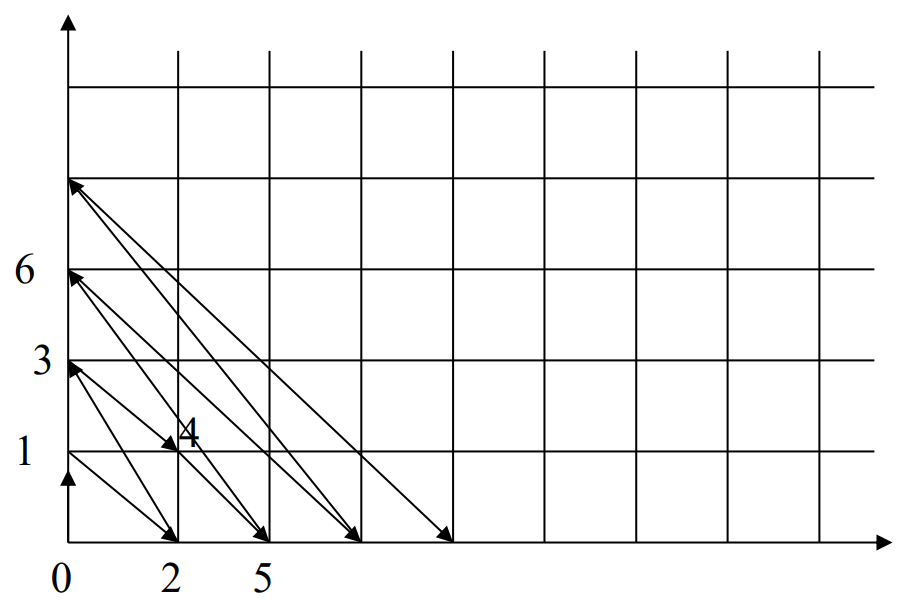
\includegraphics[width=8cm]{biiezione.png} 
    \caption{Grafico di biiezione}
  \end{figure}

  Si osservi che la funzione \(g(y,x)\) è computabile da una macchina di Turing, ossia \(\exists i\in \mathbb N : f_i=g\), ed è possibile calcolarla tramite i seguenti passaggi:
  \begin{enumerate}
    \item Si sceglie un alfabeto finito \(A\) per codificare i numeri naturali ed ogni altra informazione richiesta per la computazione;
    \item Si traduce la rappresentazione di \(n\) in un'opportuna rappresentazione della coppia \(<x,y>\) corrispondente ad \(n\). La rappresentazione decimale di \(n\) può essere tradotta nelle due rappresentazioni decimali di \(x\) ed \(y\), separate dal simbolo \(\$\);
    \item Si traduce \(y\) in un'opportuna codifica della TM \(y\)-esima \(M_y\) nella enumerazione di Gödel;
    \item Si simula la computazione di \(M_y\) su \(x\).
  \end{enumerate}

  \begin{theorem}
    Per ogni x ed ogni y, esiste e si può costruire una macchina di Turing universale in grado di calcolare \(g(y,x)=f_y(x)\)
  \end{theorem}  
  Tramite questo teorema si può affermare che è possibile creare una macchina di Turing che simuli il comportamento degli odierni calcolatori "general purpose".

  \section{Problemi Algoritmicamente Irrisolvibili}
  Come si è visto in precedenza, tutte le funzioni computabili \(f_y:\mathbb{N}\to\mathbb{N}\) si possono enumerare: questo significa che la cardinalità dell'insieme delle funzioni computabili è pari ad \(\aleph_0\), ovvero alla cardinalità dei numeri naturali \(\mathbb{N}\). L'insieme delle funzioni \(\{f:\mathbb{N}\to\mathbb{N}\}\) contiene la classe delle funzioni \(\{f:\mathbb{N}\to\{0,1\}\), in quanto \(\{0,1\}\subseteq \mathbb{N}\). Quindi, poichè \(\;|\;\{f:\mathbb{N}\to\mathbb{N}\}\;|\; \ge \;|\;\{f:\mathbb{N}\to\{0,1\}\}\;|\; = \wp (\mathbb{N}) = 2^{\aleph_0}\), si può dedurre che la cardinalità della classe delle funzioni da \(\mathbb{N}\) ad \(\mathbb{N}\) è strettamente maggiore della cardinalità della classe delle funzioni computabili: dunque, gran parte delle funzioni di \(\mathbb{N}\) non può essere calcolata. 

  Ora, quando si vuole definire una funzione si usa un linguaggio che la esprima, ovvero un sottoinsieme del monoide libero su di un determinato alfabeto finito: dunque, il linguaggio è un insieme numerabile. Si ricava quindi che la classe delle funzioni denotabili è a sua volta numerabile.

  Quando si scrive un programma, ci sono diverse proprietà che si vorrebbero garantire. Una di queste è la terminazione del programma, ovvero la garanzia che, dato un qualsiasi ingresso conforme al programma stesso, esso termini la propria computazione e non vada, dunque, in un ciclo infinito. Nella realtà, però, non è possibile garantire a priori la terminazione del programma per un generico valore in ingresso, nè decidere attraverso un algoritmo se ciò possa avvenire in corrispondenza di uno specifico valore in ingresso. Più in generale, il problema della terminazione del calcolo automatico è in generale non decidibile, nonostante tale problema sia definibile.
  Si è quindi constatato che esistono problemi definibili, ma che non possono essere risolti algoritmicamente: dunque, l'insieme dei problemi definibili contiene strettamente l'insieme dei problemi risolvibili, nonostante entrambi siano numerabili e con la stessa cardinalità.

  \begin{figure}[!h]
    \begin{center}    
      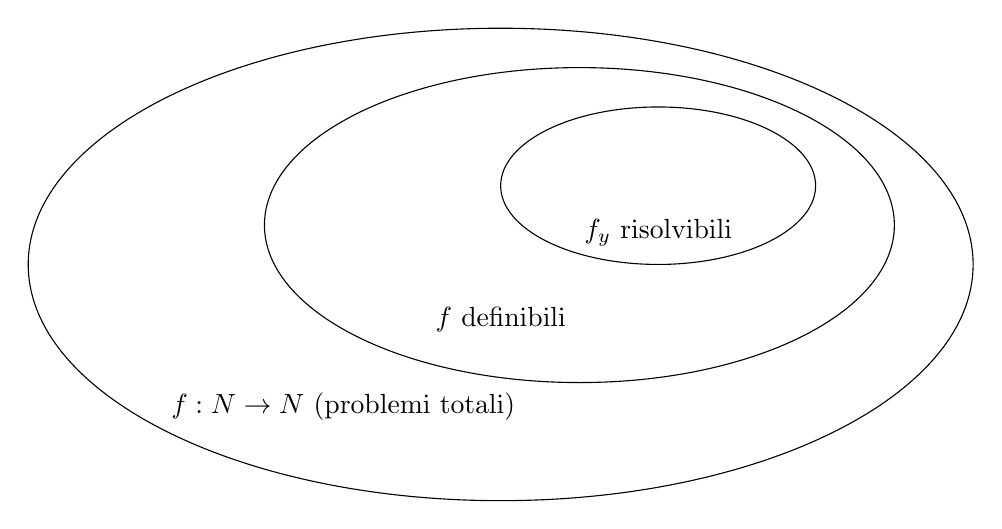
\begin{tikzpicture}
        \foreach \X [count=\Y starting from 0.75] 
        in {\(f_y\) risolvibili, \(f\) definibili, \(f:\mathbb{N}\to\mathbb{N}\) (problemi totali)} {
          \draw (-\Y,-\Y/2) circle ({2*\Y} and \Y);
          \node at (1-2*\Y,-1.1*\Y) {\X}; 
        }
      \end{tikzpicture}
    \end{center}
    \caption{Gerarchia dei problemi}    
  \end{figure}

  \begin{theorem} [Halting Problem]
    Nessuna TM può calcolare la funzione \(g:\mathbb N\times \mathbb N \to \{0,1\}\) definita nel seguente modo:
    
    \(g(x,y) = if\; f_y(x) = \bot \; then \; 1 \; else \; 0\)
  \end{theorem}

  La dimostrazione di tale teorema si ottiene tramite la tecnica della diagonale, detta anche metodo di Cantor: l'obiettivo è quello di mostrare che un'enumerazione di oggetti di cardinalità almeno 2, non è completa, ossia che un oggetto che si vorrebbe trovare all'interno di tale enumerazione in realtà non è presente. L'enumerazione di una successione può essere rappresentata come una tabella con un numero infinito di righe. L'elemento che non compare in tale tabella viene individuato per assurdo considerando inizialmente la diagonale \(d\) (dunque \(d_i\) è l'elemento che si trova all'\(i\)-esima riga e all'\(i\)-esima colonna) e poi componendo una diagonale \(d'\) tale che, per ogni \(i\), \(d'_i\) sia diverso da \(d_i\).
  
  \begin{theorem}
    Nessuna TM è in grado di calcolare la funzione totale k definita nel seguente modo:

    \(k(x)= if\;f_x(x)\neq\bot\;then\;1\;else\;0\)
  \end{theorem}

  Questo problema rappresenta un caso speciale della funzione \(g(y,x)\) in quanto \(k(x)=g(x,x)\), dunque la calcolabilità della funzione \(k\) è direttamente correlata alla calcolabilità della funzione \(g\).
  Si noti che, in generale, se un problema è irrisolvibile, può accadere che un suo caso particolare sia risolvibile, mentre una sua generalizzazione è necessariamente irrisolvibile. Al contrario, se un problema è risolvibile, può accadere che una sua generalizzazione diventi irrisolvibile, mentre un suo caso particolare rimane sicuramente risolvibile.

  Un altro teorema certamente importante è il seguente:
  \begin{theorem}
    Nessuna TM è in grado di calcolare la funzione k definita nel seguente modo:

    \(k(y)=if\; f_y(x)\neq\bot\;then\;1\;else\;0\)
  \end{theorem}
  
  Da un punto di vista pratico questo problema è interessante perchè qualifica tutti i possibili dati in ingresso. Afferma, infatti, l'irrisolvibilità del problema di decidere se un certo programma termini la propria esecuzione per qualsiasi dato in ingresso o se, al contrario, per qualche dato il programma andrebbe in loop. Nel caso precedente, invece, si era interessati al problema di sapere se un certo programma con certi dati avrebbe terminato o meno la propria esecuzione.
  
  In definitiva, si è constatato che esistono problemi non risolvibili algoritmicamente. Ciò non esclude comunque la possibilità di trovare una soluzione per tali problemi, in quanto non tutti i problemi sono risolvibili tramite un procedimento algoritmico. 

  \section{Problemi di Decisione}
  Un problema di decisione è una domanda che ha come uniche risposte si o no (0, 1). Questo può anche essere espresso come un problema di appartenenza di un determinato elemento ad un certo insieme. Più in generale si noti che una qualsiasi proprietà di un determinato elemento di un insieme può essere formalizzata come un suo sottoinsieme (ad esempio, la proprietà di terminazione del calcolo per ogni valore dei dati in ingresso individua un sottoinsieme dell'insieme di tutti i programmi). 
  
  In questa sezione si prendono in particolare considerazione i sottoinsiemi di \(\mathbb N\), indicati convenzionalmente con \(S\subseteq\mathbb{N}\). Quindi, formalmente, dato un determinato elemento \(x\in\mathbb{N}\) e un insieme \(S\), si cerca di capire se \(x\) appartenga ad \(S\).

  \begin{definition}
    La funzione caratteristica \(c_S:\mathbb{N}\to\{0,1\}\) di un insieme S è definita come segue:

    \(c_S(x)=if\;x\in S\;then\;1\;else\;0\)
  \end{definition}

  La risolvibilità del problema di appartenenza ad un insieme (detta anche ricorsività dell'insieme) dipende dalla computabilità della funzione caratteristica \(c_S\), come definito di seguito:

  \begin{definition}
    Un insieme S è ricorsivo (o decidibile) se e solo se la sua funzione caratteristica è computabile.
  \end{definition}

  Si noti, inoltre, che per ogni insieme \(S\), la sua funzione caratteristica \(c_S\) è totale: infatti, dato un qualsiasi elemento \(x\in\mathbb{N}\), questo necessariamente appartiene o non appartiene all'insieme.
  
  \begin{definition}
    Un insieme S è ricorsivamente enumerabile (o semidecidibile) se e solo se è l'insieme vuoto oppure è l'immagine di una funzione totale e computabile \(g_s\), ovvero:

    \(S=I_{g_s} = \{x\;|\;\exists y, y\in\mathbb{N} \land x=g_s(y)\}\)
  \end{definition}

  Gli insiemi decidibili devono il loro nome al fatto che il problema di appartenenza può essere risolto tramite un algoritmo meccanico e che, quindi, una TM che implementi la loro funzione caratteristica fornisce necessariamente una risposta al quesito se \(x\in S, \forall x \in \mathbb{N} \). Inoltre, per ogni insieme ricorsivamente numerabile \(S\) è possibile costruire una sequenza \(x_0=g_S(0), x_1=g_S(1), x_2=g_S(2),...\) tale per cui, se \(x\in S\), allora esiste \(i\) tale che \(x=g_S(i)\). In questo caso, esaminando la sequenza di elementi \(\{x_i\}\) si riuscirà a trovare l'elemento \(x\), concludendo che questo appartiene all'insieme \(S\). Perciò, se per un qualsiasi \(\bar{i}\) risultasse che \(x\notin\{g_S(i)\;|\;0\le i \le \bar{i}\}\) non si potrebbe concludere nè che \(x\in S\), nè che \(x\notin S\): per questo motivo, l'insieme \(S\) viene anche detto semidecidibile.

  \begin{theorem}
    Se S è ricorsivo, è anche ricorsivamente enumerabile. \\
    S è ricorsivo se e solo se sia S che \(\bar{S}=\mathbb{N}-S\) sono ricorsivamente enumerabili.
  \end{theorem}

  \break

  Quindi, riepilogando, si dice che un insieme \(S\) è:
  \begin{itemize}
    \item Ricorsivo (o Decidibile), se e solo se la sua funzione caratteristica \(c_S\) è computabile;
    \item Ricorsivamente enumerabile (o Semidecidibile), se e solo se:
    \begin{itemize}
      \item S è l'insieme vuoto;
      \item S è l'immagine di una funzione \(g_S\) totale e computabile (detta generatrice); \\ quindi, \(S=I_{g_S}=\{g_S(0), g_s(1), g_S(2),...\}\)
    \end{itemize}
  \end{itemize}

  Si consideri ora il seguente teorema:
  \begin{theorem}
    Per ogni insieme S, se \(i \in S\) implica che \(f_i\) sia totale e se per ogni funzione \(f\) totale e computabile, esiste \(i\in S\;|\;f=f_i\), allora S non è ricorsivamente enumerabile. 
  \end{theorem}

  Informalmente, questo teorema stabilisce che tutte le funzioni totali computabili non sono ricorsivamente enumerabili (mentre le funzioni parziali computabili lo sono). Dunque, tale teorema afferma implicitamente che non esiste nessun formalismo ricorsivamente enumerabile in grado di definire tutte e sole le funzioni totali e computabili: infatti, gli FSA sono in grado di definire le funzioni totali, ma non tutte, le TM definiscono tutte le funzioni computabili, ma anche quelle non totali, e un linguaggio di programmazione (come il C) è in grado di definire tutti gli algoritmi, ma anche quelli che non terminano mai. 
  
  Si cerca quindi di comprendere se sia possibile eliminare le funzioni non totali: per far ciò, si prenda in considerazione una generica funzione parziale, ad esempio, arricchendo \(\mathbb{N}\) con il valore \(\{\bot\}\) o con qualsiasi altro simbolo che indichi che la funzione non è definita per certi valori. Tale trasformazione da funzione parziale a totale, però, non può essere applicata perchè nel passaggio è possibile perdere la computabilità della funzione. Questo risultato è enunciato nel seguente teorema:
  
  \begin{theorem}
    Non esiste una funzione totale e computabile h che sia un'estensione della seguente funzione:
    \(g(x)=if\;f_x(x)\neq\bot\;then\;f_x(x)+1\;else\;\bot\)
  \end{theorem}

  Tale teorema, afferma quindi che non è possibile estendere una funzione parziale ad una totale, in quanto si potrebbe perdere la sua computabilità.

  Vale anche il seguente risultato:
  \begin{theorem}
    Un insieme S è ricorsivamente enumerabile se e solo se \(S=D_h\), in cui h è una funzione parziale e computabile (\(S=\{x\;|\;h(x)\neq \bot\}\)), oppure se e solo se \(S=I_g\), in cui g è una funzione parziale e computabile (\(S=\{x\;|\;x=g(y), y\in \mathbb{N}\}\)).
  \end{theorem}

  Quindi, dato l'insieme \(K=\{x\;|\;f(x) \neq \bot\}\) questo è semidecidibile perchè \(K=D_h\), con \(h(x)=f_x(x)\), ma è anche indecidibile in quanto la funzione caratteristica dell'insieme \(K\), definita come \(c_K(x)=if\;f_x(x)\neq \bot\;then\;1\;else\;0\), non è computabile. Si è appena dimostrato che esistono insiemi che sono semidecidibili, ma allo stesso tempo indecidibili.

  \begin{figure}[!h]
    \begin{center}    
      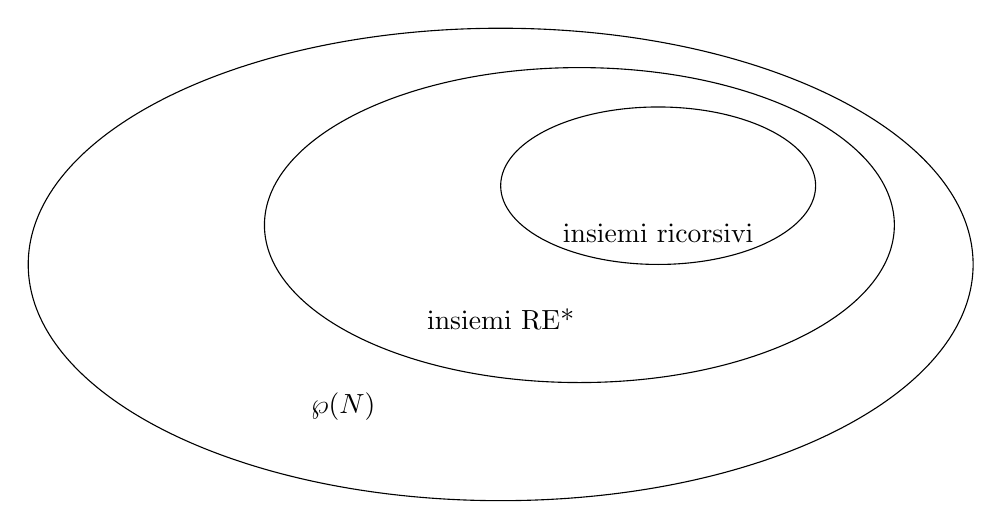
\begin{tikzpicture}
        \foreach \X [count=\Y starting from 0.75] 
        in {insiemi ricorsivi, insiemi RE*, \(\wp(\mathbb{N})\)} {
          \draw (-\Y,-\Y/2) circle ({2*\Y} and \Y);
          \node at (1-2*\Y,-1.1*\Y) {\X}; 
        }
      \end{tikzpicture}
    \end{center}
    \caption{Gerarchia degli insiemi}    
  \end{figure}

  *Con RE si indicano gli insiemi Ricorsivamente Enumerabili.

  Si noti che tutte le inclusioni sono strette.

  \section{Teoremi di Kleene e Rice}

  \begin{theorem} [Teorema di Kleene del punto fisso]
    Sia t una qualunque funzione totale e computabile. Allora è sempre possibile trovare un intero p, tale per cui:
    
    \(f_p=f_{t(p)}\)\\
    La funzione \(f_p\) è detta punto fisso di t, perchè t trasforma \(f_p\) in \(f_p\) stessa.
  \end{theorem}

  \begin{theorem}[Teorema di Rice]
    Sia F un insieme generico di funzioni computabili. L'insieme \(S=\{x\;|\;f_x\in F\}\) degli indici delle TM che calcolano le funzioni di F, è ricorsivo se e solo se \(F=\emptyset\) oppure F è l'insieme di tutte le funzioni computabili.
  \end{theorem}

  Il teorema di Rice ha un forte impatto pratico negativo, in quanto afferma che, in tutti i casi non banali, \(S\) non è decidibile. Non è quindi possibile stabilire algoritmicamente se un dato algoritmo sia in grado di risolvere un determinato problema, nè se due programmi siano equivalenti (ossia se calcolino la stessa funzione). Il grande impatto pratico del teorema di Rice deriva dal fatto che il concetto di sottoinsieme \(F\) di funzioni computabili è un'espressione formale del concetto generale di proprietà di problemi risolvibili: una proprietà degli elementi di un insieme è un sottoinsieme dell'insieme dato e una funzione computabile è una formalizzazione del concetto di problema risolvibile; quindi, il teorema di Rice afferma che non è possibile stabilire se un determinato algoritmo risolve un problema pur risolvibile che godi di una qualsiasi proprietà non banale.